\section{Syllable types}
Upon evaluating the models in Experiment I, it became clear that they do not perform equally across all classes of syllables. In particular, those prefixed with "z", such as "z-wei", appear to be more difficult for the classifiers. In this experiment, we test how well the models perform when they are trained on a subset of the syllables.

There are three main classes of syllables that appear in the data set: those prefixed with "z", "zz", and those without a prefix. We created two new data sets with the "z" and "zz" syllables filtered out, respectively. We perform a 10 fold cross validation using these filtered sets and present the AUC scores in table \ref{tab-syl-type-results}. 

\begin{table}[h]
\centering
\caption{Experimental results}
\begin{tabular}{|l|c|c|c|c|}
\hline
\multicolumn{1}{|c|}{}      &   None       &   z          &     zz      &    sh       \\ \hline
LSTM-1                      &   84.9     &   92.3    &     62.1  &             \\ \hline
LSTM-2                      &   78.3     &   90.2     &     84.5  &             \\ \hline
Bi-LSTM-1                   &   84.7     &   92.0     &     85.9  &             \\ \hline
\end{tabular}
\label{tab-syl-type-results}
\end{table}

\begin{figure*}[t]
    \centering
    \begin{subfigure}[b]{\columnwidth}
        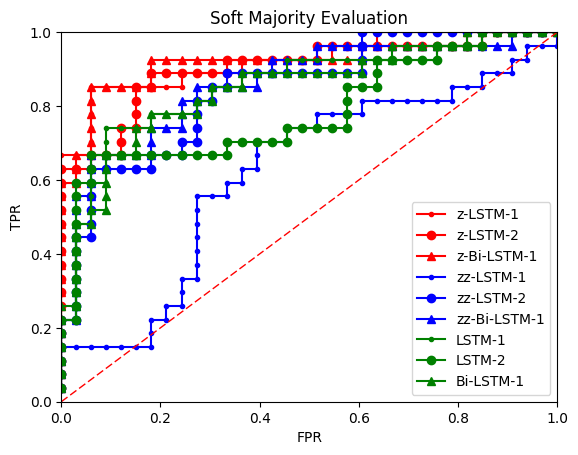
\includegraphics[width=\textwidth]{syl_type_exp-roc.png}
        \caption{}
        \label{rfidtest_xaxis}
    \end{subfigure}
    \begin{subfigure}[b]{\columnwidth}
        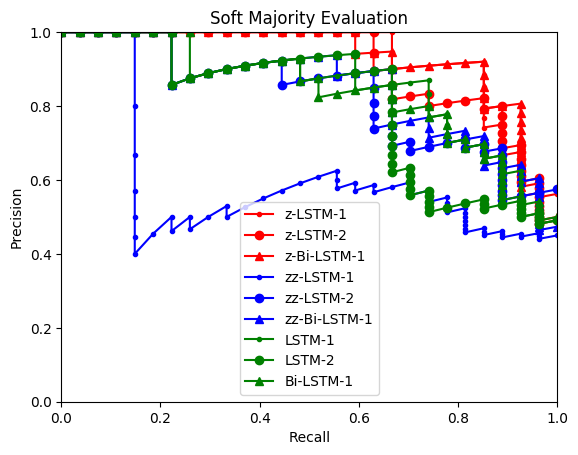
\includegraphics[width=\textwidth]{syl_type_exp-pr.png}
        \caption{}
        \label{rfidtest_yaxis}
    \end{subfigure}
\end{figure*}

Figure \ref{curves} I need to consolidate this into two graphs, an ROC and PR curve with all six models each.  

The models whose input did not include syllables prefixed with "z" performed significantly better according to their AUC scores. Models who were not trained on "zz" prefixed syllables did not fair so well, especially $LSTM-1$. In contrast, $LSTM-2$ improves when "zz" syllables are excluded from its input. 

Both the "z" and "zz" syllables contribute about the same to the number of syllables, at 27 and 76 percent. Being that all three models scored above 90 when trained without "z" syllables, it may be a wise heuristic, especially for smaller data sets such as this. This intuitively follows from the observation that, even for healthy speakers, these syllables are more difficult to pronounce correctly.
